\chapter{Evaluaci\'on de rankings sobre benchmarks}
\label{sec:evaluacion}

En esta secci\'on se presentan diversas formas de evaluar a los algoritmos propuestos en el cap\'itulo anterior. En particular, se muestra que el algoritmo de refinamiento probabil\'{i}stico con sobreespecificaci\'on es capaz de generar un ranking de ERs que es similar a la distribuci\'on de frecuencias de las ERs observadas en corpora usando m\'etricas autom\'aticas y que tambi\'en tiene un buen desempe\ ~no cuando se usan m\'etricas manuales. 

%Este cap\'itulo esta dividido en tres secciones, en la primera secci\'on se muestra un ejemplo de ranking de ERs del corpus GRE3D7 comparado con el ranking de ERs generadas por el algoritmo de refinamiento probabil\'istico, usando probabilidades de uso aprendidas desde las dem\'as im\'agenes del GRE3D7. Se comparan ambos rankings y se d\'a la presici\'on, es %decir el porcentaje de matcheo perfecto. Se muestran las ERs generadas por el algoritmo que no estan en el corpus, y se argumenta que son buenas para identificar al target igual que las dem\'as. Luego en la Secci\'on \ref{sec:compara-varias} explicamos la misma comparaci\'on pero teniendo en cuenta todas las escenas verde-azules del corpus GRE3D7 y hacemos comparaciones de rankings de ERs dadas por nuestro algoritmos con 3 diferentes distribuciones de probabilidades como entrada, contra las ERs humanas existentes en el corpus. Mostramos la entrop\'ia cruzada entre las distribuciones propuestas y la del corpus. El corpus usado para la comparaci\'on es el GRE3D7 ya que ese corpus tiene un ranking de ERs dadas por humanos para cada escena.
%, Incluso cuando no se dispone de corpus espec\'{i}fica para un objeto de destino determinado.

%Se discuten en detalle los experimentos ejecutados para la escena que se muestra en la Figura~\ref{GRE3D7-stimulus},  %(escena 3 en el corpus GRE3D7)
%a continuaci\'on, un resumen de los resultados de las otras siete escenas que utilizamos para las pruebas.
%https://docs.google.com/spreadsheets/d/1Hn2fqQZBqkJscUE62UakNsKmMKOvLodvLoAbztT6kV4/edit#gid=6 en drive

\section{Evaluaci\'on de rankings sobre el corpus GRE3D7}
\label{sec:compara}
En esta sección presentamos una evaluación cuantitativa y automática de los algoritmos en el dominio del corpus GRE3D7~\cite{gre3d7} introducido en la Seccion~\ref{sec:corpusGRE} del Capítulo~\ref{sec:seleccion}. Mostraremos una comparaci\'on con el ranking de ERs dadas por el algoritmo con las probabilidades de uso calculadas como se describe en la Secci\'on~\ref{sec:learning}, es decir con aprendizaje autom\'atico a partir de las dem\'as im\'agenes del corpus y ejecutando nuestro algoritmo 10000 veces. El algoritmo probabilístico con sobreespecificación es capaz de generar una distribución de ERs similar a la que se observa en el corpus. Describimos primero en detalle los experimentos que realizamos para la escena que se muestra en la Figura~\ref{contexto-evaluacion}, en la Sección \ref{sec:compara}. Luego, en la Sección \ref{sec:compara-varias}, resumimos los resultados obtenidos en evaluaciones similares para otras 7 escenas del corpus. 
\subsection{Caso de estudio de una escena del corpus GRE3D7}

Las probabilidades de uso aprendidas usando regresión lineal como se muestra en el Capítulo~\ref{sec:learning} se muestran en \ref{probabilidades-escena2}, y ejecutando el algoritmo 10000 veces.

\begin{table}[H]
\begin{center}
\footnotesize{
\begin{tabular} {  l c c c c c c c c c c}
\hline
%\multicolumn{1}{c}{}
%&\multicolumn{1}{c}{Domain}
%&\multicolumn{3}{c}{Descriptions}\\

R				&{\it ball}			& {\it cube}	& {\it green}	  & {\it blue} & {\it large} & {\it small} & {\it top} & {\it front} & {\it left} & {\it ontop}   \\
\hline
R.\puse	& 1.0			& 1.0		& & &  &   &  & & & \\
\hline

\end{tabular}
}
\end{center}
\vspace*{-.5cm} 
\caption{Distribuci\'on de probabilidad de las propiedades y relaciones de la figura de ejemplo.}\label{probabilidades-escena2}

Obtuvimos 14 expresiones referenciales diferentes para la escena de la Figura~\ref{contexto-evaluacion}, el corpus tiene 12 ERs diferentes generadas por personas para esa escena. Es interesante ver que aunque es posible generar cientos de ERs para esta escena, el algoritmo, guíado por las probabilidades de uso, genera sólo 14 ERs en 10000 ejecuciones. Además, el algoritmo genera, para esta imagen, 2 ERs con alta frecuencia (la bola verde y la bola verde pequeña representan el 98% de las ERs generadas automáticamente) y otras ERs con una frecuencia mucho menor (representan el 2% de las ERs generadas). Estas 2 ERs más frecuentes generadas por el algoritmo coincide con las 2 ERs más frecuentes generadas por las personas (la bola verde y la bola verde pequeña representan el 81% de las ERs generadas por humanos para la imagen). 
 
\begin{figure}[!ht]
\centering
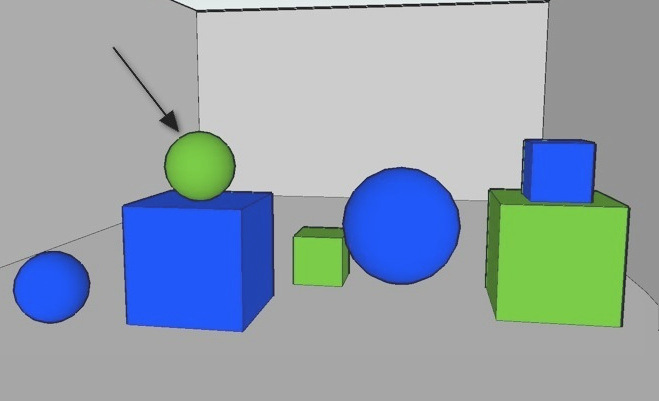
\includegraphics[width=.6\textwidth]{images/3.jpg}\\[0pt]
\label{fig-GRE3D7}
\caption{Imagen del GRE3D7 corpus.}\label{contexto-evaluacion}
\end{figure}

La \textbf{precisi\'on}  es una m\'etrica autom\'atica estricta que se puede usar para comparar rankings de ERS. Es la proporci\'on de coincidencias perfectas entre la salida de algoritmo y las ERs generadas por humanos y encontradas en corpora. 
La primer comparaci\'on de rankings de ERs se muestra en la Tabla \ref{results-algo-fig3}. Para cada ER, indicamos el n\'umero de veces que aparece en el corpus (\#Cor), la proporci\'on que representa (\%Cor), el n\'umero de veces que la gener\'o nuestro algoritmo (\#Alg) y la proporci\'on que representa (\%Alg).
Por \'ultimo, la precisi\'on (\%Acc) nos d\'a el porcentaje de aciertos de las ERs generadas por el algoritmo y se calcula como el m\'inimo entre el \%Cor y \%Alg. 

\begin{table}[H]
\begin{small}
\begin{center}
\begin{tabular}{|l|r|r|r|r|r|}
\hline
\multirow{2}{*}{Expresiones Referenciales} & \multicolumn{2}{|c|}{Corpus} & \multicolumn{2}{|c|}{Algoritmo} & Precisi\'on \\ \cline{2-6} 
 & \#Cor & \multicolumn{1}{|c|}{\%Cor} & \multicolumn{1}{|c|}{\#Alg} & \multicolumn{1}{|c|}{\%Alg} & \multicolumn{1}{|c|}{\%Acc} \\
\hline
ball, green                                    & 91 & 65.00 & 6376 & 63.76 & 63.76 \\
ball, green, small                              & 23 & 16.43 & 3440 & 34.40 & 16.43 \\
ball, green, small, ontop(blue, cube, large)      &  8 &  5.71 &    0 &  0.00 &  0.00\\
ball, green, ontop(blue, cube)                  &  5 &  3.57 &    0 &  0.00 &  0.00\\
ball, green, ontop(blue, cube, large)            &  5 &  3.57 &    0 &  0.00 &  0.00\\
ball, green, small, ontop(blue, cube)            &  2 &  1.43 &    0 &  0.00 &  0.00\\
ball, ontop(cube)                             &  1 &  0.71 &   27 &  0.27 &  0.27 \\
ball, green, small, ontop(blue, cube, large, left) &  1 &  0.71 &    0 &  0.00 &  0.00\\
ball, small, ontop(cube,large)	              &  1 &  0.71 &    2 &  0.02 &  0.02 \\
ball, green, top                                &  1 &  0.71 &    0 &  0.00 &  0.00\\
ball, small, ontop(cube)                       &  1 &  0.71 &    3 &  0.03 &  0.03 \\
ball, green, ontop(cube)                       &  1 &  0.71 &    0 &  0.00 &  0.00\\
ball, front, green                              &  0 &  0.00 &   97 &  0.97 &  0.00\\
ball, front, green, small                        &  0 &  0.00 &   13 &  0.13 &  0.00\\
ball, front, top                                &  0 &  0.00 &   12 &  0.12 &  0.00\\
ball, green, left	                              &  0 &  0.00 &   11 &  0.11 &  0.00\\
ball, top                                      &  0 &  0.00 &   10 &  0.10 &  0.00\\
ball, green, left, small                         &  0 &  0.00 &    5 &  0.05 &  0.00\\
ball, left, top                                 &  0 &  0.00 &    2 &  0.02 &  0.00\\
ball, small, top                                &  0 &  0.00 &    1 &  0.01 &  0.00\\
ball, front, ontop(cube, left)                  &  0 &  0.00 &    1 &  0.01 &  0.00\\

\hline
Total & 140 & 100 & 10000 & 100 & 80.51 \\
\hline
\end{tabular}
\caption{ERs del corpus, y las producidas por nuestro algoritmo para la Figura~\ref{contexto-evaluacion}.\label{results-algo-fig3}}
\vspace*{-.5cm}
\end{center}
\end{small}
\end{table}

 La precisi\'on del algoritmo con respecto al corpus GRE3D7 para esta escena es del 80\%. De las 14 ERs diferentes generadas por el algoritmo, 5 se encuentran en el corpus y las otras 9 no. Estas 9 expresiones referenciales incluyen propiedades de ubicación del target no con respecto a un landmark si no a su posición en la escena 3D. Por ejemplo \emph{la espera verde que está a la izquierda} se refiere a que la esfera verde está a la izquierda de la escena.  La probabilidad de uso de este tipo de propiedades es menor al 1 \%, en particular la de left es 0,007, pero, como esa probabilidad no es cero, dichas propiedades aparecen en ERs (siempre con menos de un 1% de frecuencia).  La m\'etrica de precisi\'on ha sido utilizada en trabajos anteriores para comparar la salida de un algoritmo de generaci\'on de ER con las ERs que se encuentran en corpora~\cite{sluis07:eval,viet:gene11} y se considera una m\'etrica muy estricta para esta tarea.

\subsection{Evaluaci\'on emp\'irica sobre el resto del corpus}
\label{sec:compara-varias}

Como es habitual cuando hacemos una evaluaci\'on con un caso particular, podemos pensar, que como el algoritmo tiene un componente de azar, por eso nos di\'o bastante bien, para esa ejecuci\'on particular. Por eso aqu\'i se muestra la misma comparaci\'on realizada en la secci\'on anterior pero con todas las im\'agenes verde-azules del corpus GRE3D7. 
Para enriquecer esta parte mostraremos otros baselines, los cuales dos dar\'an pistas de que las probabilidades de uso aprendidas con el m\'etodo que presentamos en esta tesis son \'utiles para aproximar al ranking de ERs que aparece en corpora. Los baselines que se presentan ejecutan el algoritmo con una distribuci\'on aleatoria de probabilidades de uso, y con una distribuci\'on uniforme (en las ERs tomando tanto las generadas por el sistema como las del corpus y las generadas como el modelo aleatorio). El Top baseline, es en el que el algoritmo us\'o las probabilidades de uso sacadas del corpus mismo. 

\begin{table}[h!]
\begin{small}
\begin{center}
\begin{tabular}{|l|c|c|c|c|}
\hline
         &  \puse\ de escena & \puse\ aprendidas & \puse\ random & uniforme \\ \hline
Escena 1	&	85.75\%	&	84.49\%	&	17.95\%	&	5.37\%	\\
Escena 3	&	82.81\%	&	80.51\%	&	9.89\%	&	4.40\%	\\
Escena 6	&	90.11\%	&	83.30\%	&	4.13\%	&	4.16\%	\\
Escena 8	&	86.52\%	&	64.06\%	&	16.32\%	&	9.75\%	\\
Escena 10	&	89.49\%	&	75.80\%	&	7.56\%	&	3.70\%	\\
Escena 12	&	80.21\%	&	81.29\%	&	57.09\%	&	6.68\%	\\
Escena 13	&	89.98\%	&	50.79\%	&	9.30\%	&	3.59\%	\\
Escena 21	&	92.13\%	&	80.01\%	&	8.45\%	&	6.77\%	\\
\hline
Promedio	&	87.13\%	&	75.03\%	&	16.34\%	&	5.55\%	\\

\hline
\end{tabular}
\caption{Precisi\'on entre las ERs del corpus y las generadas usando valores de \puse\ calculados desde la escena, aprendidos autom\'aticamente, provenientes de distribuciones random y uniformes.}\label{results-algo-all}
\end{center}
\end{small}
\end{table}


La primera columna muestra los valores obtenidos cuando corremos el algoritmo sobre la escena
con los valores de \puse\ obtenidos~\emph{de la propia escena}. Como se puede esperar,
esta columna tiene el mayor promedio de precisi\'on.

La segunda columna muestra los resultados del algoritmo cuando se ejecuta con \puse\ aprendido de
corpora como se explica en la Secci\'on~\ref{sec:learning} del cap\'itulo anterior. Este es el caso m\'as interesante porque muestra la capacidad de nuestra propuesta de generalizar a escenas no vistas con anterioridad y para las que no hay corpus. Para la mayor\'{i}a de las escenas la precisi\'on
es mayor al 80\% y la precisi\'on promedio es 75\%. La relativamente baja precisi\'on
obtenida en la escena 13 se explica principalmente las pobres estimaciones del valor de~\puse\ para las palabras \emph{large} y \emph{small} que son propiedades vagas y no absolutas ya que dependen de cu\'an grandes son en relaci\'on con los otros elementos del contexto.  

En el corpus, las relaciones \emph{large} y \emph{small} se utilizan mucho m\'as cuando el target no puede ser identificado usando s\'olo propiedades taxon\'omicas (\emph{ball} y \emph{cube}) y propiedades absolutas (\emph{green} y \emph{blue}), pero las caracter\'{i}sticas que hemos utilizado para el aprendizaje autom\'atico no capturan dichas dependencias como se discute en la Secci\'on \ref{sec:learning-corpus} del Cap\'itulo \ref{sec:algoritmo}.

A pesar de esta limitaci\'on, el promedio de la segunda columna es 75\%. Para una m\'etrica como la de precisi\'on que es considerada demasiado estricta, estos resultados son buenos. Adem\'as, el 25\% no cubierto por el algoritmo puede contener ERs igualmente buenas como evaluamos en la Secci\'on \ref{sec:humanevaluation}. Uno podr\'ia argumentar entonces que los valores de \puse\ aprendidos a partir del corpus son lo suficientemente buenos para ser utilizados para generar REs para nuevas escenas del dominio.

Las dos \'ultimas columnas pueden ser consideradas como baselines. En la primera generamos
valores aleatorios para \puse\. La precisi\'on obtenida es en la mayor\'{i}a de los casos pobre, pero con
una variaci\'on notable debido al azar. Adem\'as estas ejecuciones toman mucho m\'as tiempo en finalizar, lo que indica que se est\'an realizando demasiadas particiones sin conseguir llegar a la meta. Esta observaci\'on de performance es consistente con los resultados de los experimentos de generaci\'on humana realizados por \cite{keysar:Curr98,} y discutidos en la Seccion \ref{sec:psicolinguistica} del Cap\'itulo \refsec:seleccion}. Keysar argumenta que, las personas usan la prominencia de las propiedades en el dominio como heur\'istica para guiar la generaci\'on de ERs de forma de disminuir la carga cognitiva de tener que probar con todas las propiedades del dominio. Si la heur\'istica es buena, en muchos casos no es necesario ``revisar'' la ER para que identifique un\'ivocamente al target. Como efecto colateral de este proceso heur\'istico la ER resultante puede estar sobreespecificada, pero se genera r\'apidamente.  

Adem\'as de poca precisi\'on, cuando se utilizaron probabilidades random,  muchas de las ERs generadas suenan poco natural y son dif\'iciles de realizar sin introducir ambig\"uedades como, por ejemplo, (\textit{peque\~na cosa sobre
el cubo azul que est\'a abajo de algo que es peque\~no}). En la \'ultima columna se presenta la precisi\'on de una corrida artificial, le llamamos uniforme, uniforme tomando todas las ERs de las dem\'as columnas y asign\'andoles la misma probabilidad.
Para comparar nuestros resultados colos 3 baselines usamos tambi\'en entrop\'ia cruzada.
En teor\'ia de la informaci\'on, la \textbf{entrop\'ia cruzada} entre dos distribuciones de probabilidad mide la media de bits necesarios para identificar un evento de un conjunto de posibilidades, si un esquema de codificaci\'on est\'a basado en una distribuci\'on de probabilidad dada q, m\'as que en la verdadera distribuci\'on p. Vamos a comparar la entrop\'ia cruzada entre la distribuci\'on de probabilidad que se encuentra en el corpus, y la distribuci\'on de ER del corpus y las de ejecuciones del algoritmo con las probabilidades que acabamos de describir~(ver~\cite{juraksky:spee08} para obtener detalles sobre evaluaci\'on de entrop\'{i}a cruzada). En la Figura~\ref{Entropy} se muestran los resultados para las ocho escenas que hemos considerado.

\begin{figure}[ht]
\centering
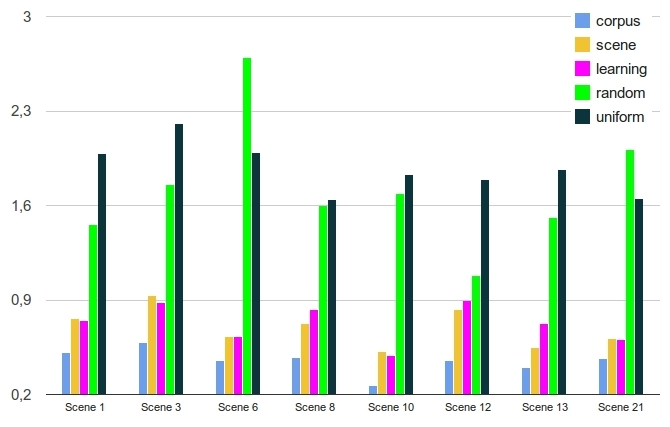
\includegraphics[width=0.6\textwidth]{images/entropy.jpg}
\caption{Entrop\'ia cruzada entre la distribuci\'on del corpus y diferentes ejecuciones del algoritmo.}\label{Entropy}
\end{figure}
  
Las entrop\'{i}as cruzadas de las dos primeras ejecuciones (\emph{escena} y \emph{aprendizaje autom\'atico}) son, en general, mucho m\'as cercanas de la entrop\'{i}a del corpus, que las entrop\'ias cruzadas de \emph{random} y \emph{uniforme}. S\'olo en la escena 12 random, por azar se acerca un poco m\'as.

%En esta secci\'on presentamos dos evaluaciones diferentes que realizamos en nuestro algoritmo. Secci\'on~\ref{sec:automaticevaluation} describe una evaluaci\'on con respecto al estado del arte~\cite{KrahmerGRAPH}. GRAPH fue el de mejor desempe\~no en las dos ediciones de la competencia ASGRE~\cite{gatt-balz-kow:2008:ENLG}. Debido a las limitaciones de los indicadores autom\'aticos, en la Secci\'on~\ref{sec:humanevaluation} realizamos una evaluaci\'on humana en la que pedimos a jueces humanos comparar la salida producida por nuestro algoritmo con las expresiones producidas por los seres humanos (las del corpus).


\section{Evaluaci\'on de rankings en el TUNA Challenge} \label{sec:automaticevaluation}

En esta secci\'on se presenta la comparaci\'on de nuestro algoritmo con el algoritmo que tuvo el mejor desempe\~no en el TUNA Challenge. 

\subsection{El TUNA Challenge}
El TUNA Challenge ...

El algoritmo GRAPH que describimos en el Cap\'itulo \ref{sec:seleccion} es un algoritmo determin\'stico y por lo tanto produce la misma expresi\'on referencial cuando se ejecuta con el mismo target y contexto. Nuestro algoritmo es no-determin\'istico, puede dar una expresi\'on referencial diferente cada vez que se ejecuta. Con el fin de compararlos corremos nuestro algoritmo 100 veces y hacemos un ranking de las 20 ERs ordenadas por la frecuencia que se produjeron. Utilizamos la parte de prueba del corpus TUNA (el cual fue introducido en la Secci\'on \ref{sec:corpusTUNA}), para comparar el ranking de ERs dado por nuestro algoritmo con las salidas del algoritmo GRAPH cuyos resultados se describen en~\cite{KrahmerGRAPH} y se reproducen en la Tabla~\ref{Tabla_sis_1_20}.


\subsection{Comparaci\'on con el TUNA Challenge}
El algoritmo GRAPH define la generaci\'on de expresiones referenciales como un problema de b\'usqueda en un grafo, devuelve el grafo distintivo de menor costo (si existe) dada una funci\'on de costo particular. Comparamos a este algoritmo usando las m\'etricas precisi\'on, Dice y \textsc {masi}, introducidas en la Secci\'on \ref{sec:metricasAutomaticas}. 

Recordemos que el corpus TUNA tiene 2 partes, una parte cuyo dominio son muebles, y otra parte cuyo dominio son personas, ambos ubicados en una grilla. Para realizar esta comparaci\'on se us\'o s\'olamenta la parte singular del corpus.

En la Tabla~\ref{Tabla_sis_1_20} mostramos m\'etricas autom\'aticas y comparamos la performance de nuestro sistema con el sistma GRAPH para la primer ER en el ranking y para las primeras 20 ERs del ranking.

\begin{table}[H]
\begin{center}
\begin{tabular}{|l|c|c|c|}
\hline
%Figure & Model \puse &  Learning \puse & Random \puse &  Uniform \puse \\
	 	& 	Dice		&	\textsc{masi}	&	Precisi\'on		\\
\hline
sistema GRAPH, Dominio muebles	& 	80\% 		&	59\%	&	48\%		 	\\
sistema GRAPH, Dominio personas 	& 	72\%		&	48\%	&	28\%			\\
\hline
Nuestro sistema, Dominio muebles (top 1)	&	80\%		&	60\%	&	47\%		\\
Nuestro sistema, Dominio personas (top 1)	&	65\%		&	37\%	&	19\%		\\
\hline
Nuestro sistema, Dominio muebles (top 20)&	87\%		&	75\%  	&	65\%		\\
Nuestro sistema, Dominio personas (top 20)   &	81\%		&68\%	&	60\%		\\
\hline
\end{tabular}
%\vspace*{.1cm}
\caption{Comparaci\'on del algoritmo GRAPH y nuestro sistema. Consideramos 3 m\'etricas autom\'aticas para el top 1 y para el top 20 ERs producidas por nuestro algoritmo.}
%\vspace*{-.5cm}
\label{Tabla_sis_1_20}
\end{center}
\end{table}
%\vspace*{-.5cm}
%Accuracy, Dice and \textsc{masi} assess humanlikeness with respect to a corpus of human referring expressions. In the Figure~\ref{graficoPresicion} the accuracy for our system and the GRAPH system is compared. The left GRAPH corresponds to the furniture domain and the right GRAPH corresponds to the people domain. We can see that taking the top 1 ER our system accuracy is lower than GRAPH performance for the people domain. However, if we consider the top 20 REs that our algorithm is able to produce we can see that the accuracy for both domains gets higher than 60\%. This shows that our algorithm is able to generate REs that are more similar to those produced by humans than the GRAPH algorithm, although these REs are not ranked first. 

%Another result that we can observe is that the people domain accuracy is much lower for the top 1 ER than for the furniture domain (19 vs 47), but the accuracy stabilizes when REs lower in our ranking are considered. This may be explained by the fact that the training set for the people domain is smaller and less balanced and hence, the probabilities of use inferred do not generalize as well as in the furniture domain. 

%\hline
%Precisi\'on, Dice y \textsc{masi}  evaluar humanlikeness con respecto a un corpus de expresiones humanas en referencia.
En la Figura~\ref{graficoPresicion} se muestra una comparaci\'on entre la precisi\'on de nuestro sistema y el sistema GRAPH. El gr\'afico de la izquierda corresponde al dominio muebles y el gr\'afico de la derecha corresponde al dominio personas. En el dominio muebles estamos obteniendo casi los mismos n\'umeros en las m\'etricas evaluadas.
Podemos ver que si tomamos la parte superior, es decir 1 ER (la primera, la m\'as probable), nuestra precisi\'on es menor que de GRAPH para el dominio de las personas. Sin embargo, si tenemos en cuenta las 20 mejores ERs que nuestro algoritmo es capaz de producir, podemos ver que la precisi\'on para ambos dominios se hace mayor del 60\% (60\% para personas y 65\% para muebles). Esto demuestra que nuestro algoritmo es capaz de generar ERs que son m\'as similares a las producidas por los seres humanos que el algoritmo GRAPH, aunque estas ERs no esten en primer lugar. Si el algoritmo GRAPH fuera modificado para ser no-determin\'istico es posible que tambi\'en mejorara su precisi\'on en 20 o m\'as ejecuciones. Esta es una l\'inea interesante de trabajo futuro. 

\begin{figure}[H]
\begin{minipage}{0.50\linewidth}
\centering
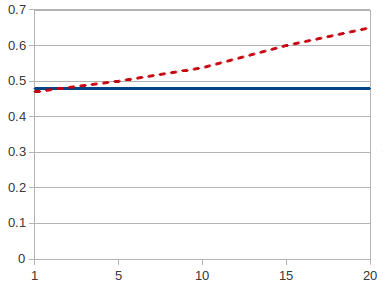
\includegraphics[width=\textwidth]{images/furniturePrec.png}
\caption{Muebles.}
%\end{figure}
\end{minipage}
%\begin{figure}[ht]
\begin{minipage}{0.50\linewidth}
\centering
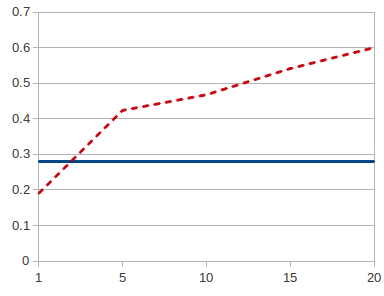
\includegraphics[width=\textwidth]{images/precP.png}
\caption{Personas.}
\end{minipage}
\caption{Comparaci\'on de la precisi\'on  del algoritmo GRAPH y nuestro sistema. El eje x indica que la precisi\'on se calcul\'o teniendo en cuenta las x primeras ER en el ranking. El eje y indica la precisi\'on . Nuestro sistema es representado como una l\'inea de puntos y GRAPH como una l\'inea continua.\label{graficoPresicion}}
\end{figure}

Otro resultado que podemos observar es que la precisi\'on  del top 1 en el dominio personas es mucho menor (19\%) que para el dominio de muebles (47\%), pero la precisi\'on se estabiliza cuando se consideran m\'as ERs de nuestro ranking. Esto puede explicarse por el hecho de que el conjunto de el dominio de personas contiene muchas m\'as propiedades que se pueden elegir para describir a las personas que las que contiene el dominio de muebles.

Normalmente las m\'etricas autom\'aticas tienen la desventaja de calificar como malas a ERs que son buenas ERs, es decir identifican el target un\'ivocamente, en el contexto considerado, pero las consideran malas por no ser exactamente como las que aparecen en corpora. Otra manera de evaluar qu\'e tan buena es una ER es con evaluaciones manuales. Mostraremos una evaluaci\'on humana en la siguiente secci\'on.

 
%\vspace*{-1.0cm}

\section{Evaluaci\'on humana} \label{sec:humanevaluation}

%We asked two native speaker judges of English to evaluate our referring expressions via an experiment on the web. The authors of the paper did not participate during the evaluation. The judges could register to the evaluation system so that they did not have to complete it in one go, the could come back to it later. During the evaluation we showed each judge the scenes and two randomly ordered REs. One ER corresponded to the ER present in the corpus and produced by a person and the other ER corresponded to the top 1 ER produced by our system. We asked the judges to select the ER that would be more useful to identify the target in the scene. That is, to select it from among the other objects in the stimulus pictures. 

%Our goal is to show that even if the ER generated by our algorithm does not coincide with the ER produced by a human in the corpus collection, it can be judged as good or even better than the REs generated by humans. 

%In Table~\ref{system-versus-human} we show the results from the human evaluation experiment.
%The REs produced by the system were considered equal or better by both
%judges in 60 \% of the cases and, by at least one judge in 92\% of the cases.


En las secciones anteriores describimos evaluaciones autom\'aticas de nuestro algoritmo. En esta secci\'on explicamos una evaluaci\'on humana que hicimos de las ERs generadas por nuestro algoritmo con las probabilidades de uso aprendidas para el TUNA corpus y descriptas en la secci\'on anterior.  

Como las ERs que generamos las generamos para el idioma ingl\'es, pedimos a dos jueces nativos de Ingl\'es evaluar nuestras expresiones referenciales a trav\'es de un experimento en la web. Los jueces podr\'{i}an entrar en el sistema de evaluaci\'on varias veces, es decir no ten\'ian que terminar la evaluaci\'on en la primera vez, para cada ER pod\'ian resolverla o pod\'ian volver a ella m\'as tarde. 

Durante la evaluaci\'on mostramos a cada juez una escena y dos ERs ordenadas al azar. Una ER correspond\'ia a la ER presente en el corpus TUNA producida por una persona para la escena y la otra ER correspond\'ia a la ER producida por nuestro sistema. Solicitamos a los jueces seleccionar la ER que ser\'{i}a m\'as \'util para identificar el target en la escena. El juez pod\'ia elegir una ER o indicar que las 2 ER le parec\'ian igualmente buenas.

Nuestro objetivo es mostrar que incluso si la ER generada autom\'aticamente no coincide con la ER producida por un ser humano del corpus, puede ser juzgada como buena o incluso mejor que la ER generada por una persona.

En la Tabla~\ref{system-versus-human} se muestran los resultados del experimento de evaluaci\'on humana.
Las ERs producidas por el sistema en el top 1 fueron consideradas igual o mejor por los 2 jueces que las generadas por personas en el 75\% de los casos para los muebles y en el 43\% para las personas. Esto contrasta con el 47\% para personas y 19\% para muebles de la Tabla \ref{Tabla_sis_1_20}. Esto muestra que la m\'etrica de precisi\'on es demasiado estricta para la tarea, y las m\'etricas de DICE o masi se acercan m\'as a evaluaciones humanas. Adem\'as al menos 1 juez consider\'o que el 97\% de las ERs del sistema eran tan buenas o mejores que las humanas para los muebles y (87\% para las personas). Esto muestra que la evaluaci\'on de la calidad de las ERs es parcialmente subjetiva. S\'olo en el 8\% de los casos ambos jueces coincidieron que una ER generada autom\'aticamente era peor que la humana.

\begin{table}[h!]
\begin{center}
\begin{tabular}{|l|c|c|c|}
\hline
%total scenes in evaluation set &                           80   &             68
 & Dominio muebles & Dominio personas & Media ponderada \\
\hline
%sistema igual al humano  	&	.46	&	.19	&	.33 \\
%sistema mejor por 2 jueces &	.29 	& 	.24 	& 	.27 \\
%sistema mejor por 1 or 2 jueces & .51	&	.68	&	.59 \\
sistema igual o mejor por 2 jueces  &.75  &       .43	&       .60 \\
sistema igual o mejor por 1 juez  &.97	&	.87	&	.92 \\
sistema peor por 2 jueces &	.03	&	.13	&	.08 \\
\hline
\end{tabular}
%\vspace*{.1cm}
\caption{Comparaci\'on de ERs generadas por personas y por nuestro algoritmo para el corpus TUNA.} 
\label{system-versus-human}
\vspace*{-.5cm}
\end{center}
\end{table}

%Below, we illustrate the evaluation experiment by showing examples of cases in which the system expression was considered better by both judges, by only one judge or by neither of them. 

%Figure~\ref{smallBlueFan} illustrates a case in which the human generated an underspecified ER while the system produced an ER which unequivocally identifies the target. The ER generated by the system for this figure is ``small blue fan'' while the ER produced by the human is ``blue fan''. The human ER fails to uniquely identify the target and is then not preferred by the human judges. Humans are known for producing underspecified REs which may be due to cognitive limitations for not being able to consider the whole referential context at the same time. Our algorithm is able to consider the whole referential context and combine this ability with the probability of use of the REs learned from humans. 

A continuaci\'on, se ilustra el experimento de evaluaci\'on, mostrando ejemplos de casos en los que la expresi\'on del sistema fue considerada mejor por ambos jueces, por un solo juez o por ninguno de los dos.

Figura~\ref{smallBlueFan} ilustra un caso en el que el humano genera una ER subespecificada mientras que el sistema produce un ER que identifica de manera inequ\'{i}voca al target. La ER generada por el sistema para esta figura es {\it peque\~no ventilador azul}, mientras que la ER producida por el ser humano es {\it ventilador azul}. La ER del humano no logra identificar de forma \'unica el target y entonces no es preferida por los jueces humanos. Los seres humanos son conocidos por producir ERs subespecificadas, esto puede ser debido a las limitaciones cognitivas por no ser capaz de considerar todo el contexto referencial al mismo tiempo. Nuestro algoritmo es capaz de considerar todo el contexto referencial y combinar esta capacidad con la probabilidad de uso de las ERs aprendidas de los seres humanos.




\begin{figure}[h]
\begin{minipage}{0.48\linewidth}
\centering
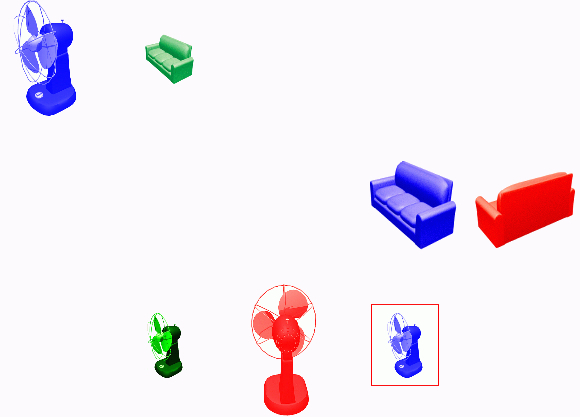
\includegraphics[width=\textwidth]{images/smallBlueFan.jpg}
\caption{Escena usada durante la recolecci\'on del TUNA corpus. La ER humana \emph{ventilador azul}, y la del sistema \emph{ventilador azul peque\~no}. Los jueces prefirieron la ER generada por el sistema.}
\label{smallBlueFan}
\end{minipage}
\hspace*{.04cm}
\begin{minipage}{0.48\linewidth}
\centering
\vspace*{.4cm}
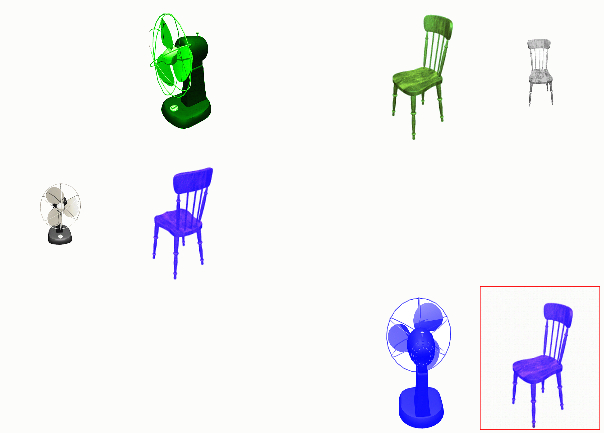
\includegraphics[width=\textwidth]{images/tuna.jpg} % esta es la 101t5 la que mostramos al principio
\vspace*{-.4cm}
\caption{Escena usada durante la recolecci\'on del TUNA corpus. La ER humana \emph{silla azul frontal}, y la del sistema \emph{La silla azul de abajo}. Ambos jueces humanos prefirieron la generada por el sistema.}
\label{BlueChair}
\end{minipage}
\end{figure}


%In Figure~\ref{BlueChair} the human ER was ``blue frontal chair'', and the system ER was ``the blue chair in the bottom''; both judges selected the system RE. This case can be explained by the fact that, in this domain, the property ``bottom'' helps more during the identification than the property ``frontal'' because it concentrates the attention of the interpreter in the lower part of the scene. Our system learns this fact by learning a higher value of \puse~for ``bottom'' than for ``frontal'' from the training data. 

En la Figura~\ref{BlueChair} la ER humana era {\it silla frontal azul}, y la ER sistema era {\it la silla azul de abajo}; ambos jueces seleccionaron la ER sistema. Este caso se puede explicar por el hecho de que, en este \'ambito, la propiedad {\it abajo} ayuda m\'as durante la identificaci\'on de la propiedad {\it frontal} porque concentra la atenci\'on del interlocutor en la parte inferior de la escena. Nuestro sistema aprende este hecho por el aprendizaje de un mayor valor de \puse\ para {\it abajo} que para {\it frontal} a partir de los datos de entrenamiento.

\begin{figure}[h]
\begin{minipage}{0.48\linewidth}
\centering
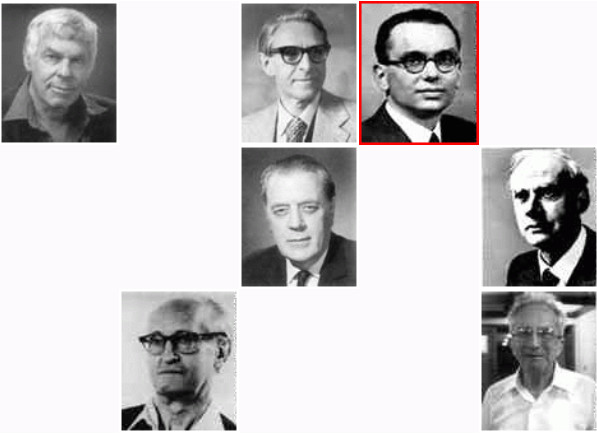
\includegraphics[width=\textwidth]{images/s59t26.jpg}
\caption{Escena usada durante la recolecci\'on del TUNA corpus. La ER humana \emph{the man with black hair}, y la del sistema \emph{the man wearing glasses in the fourth column}. Los jueces prefirieron la ER humana.}
\label{s28t25}
\end{minipage}
\hspace*{.04cm}
\begin{minipage}{0.48\linewidth}
\centering
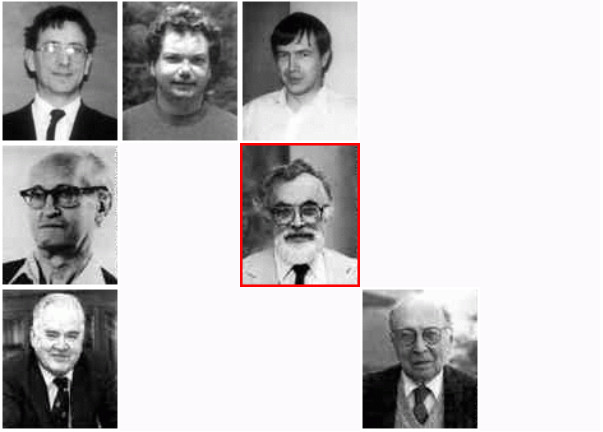
\includegraphics[width=\textwidth]{images/s315t21.jpg}
\vspace*{-.3cm}
\caption{Escena usada durante la recolecci\'on del TUNA corpus. La ER humana \emph{man with a beard},  y la del sistema \emph{man with a beard wearing glasses}. Los jueces no estuvieron de acuerdo en su preferencia.}
\label{s307t21}
\end{minipage}
\end{figure}

%Figure~\ref{s28t25} is an example for which both judges preferred the human expression. The human  ER was ``the man with black hair'', and the system's ``the man wearing glasses in the fourth column''. This example makes evident the fact that, in the people domain some properties are more salient in some images than in others because of different shades of colors. Gradable properties such as this ones (in contrast to absolute properties) are still an open problem for GRE algorithms. 

%Figure~\ref{s307t21}~illustrates a case in which the system ER was more overspecified than the human RE; the system included ``wearing glasses'' while the human did not. In this case one human subject preferred the system ER and the other the human RE. The amount of overspecification is a subjective matter where human themselves disagree. Further evaluation where REs are actually used for a task would be interesting to investigate this issue.  


Figura~\ref{s28t25} es un ejemplo en el que ambos jueces prefirieron la expresi\'on humana. La ER humana era {\it el hombre con el pelo negro}, y del sistema de {\it el hombre con gafas en la cuarta columna}. Este ejemplo pone de manifiesto el hecho de que, en el dominio de las personas algunas propiedades son m\'as destacadas en algunas im\'agenes que en otrosadebido a diferentes tonos de colores. Propiedades graduables como estas (en contraste con las propiedades absolutas) son todav\'{i}a un problema abierto para los algoritmos de GER.

Figura~\ref{s307t21}~ilustra un caso en el que la ER del sistema era m\'as sobreespecificada que la ER humana; el sistema incluye {\it con gafas}, mientras que el ser humano no lo hizo. En este caso un sujeto humano prefiere la ER del sistema y el otro la ER del humano. La cantidad de sobreespecificaci\'on es una cuesti\'on subjetiva, donde los humanos mismos no est\'an de acuerdo. Una evaluaci\'on donde las ERs se utilicen para resolver una tarea ser\'{i}a interesante para investigar este asunto.

\section{}


